
There are many analytical solutions for buried bodies of simple shape.
Hereafter are the most common ones:

%...................................
\subsubsection{Buried sphere (3D)}

To calculate the pull of gravity, we can use the fact that a sphere has the same
gravitational pull as a point mass located at its centre. The distance between 
the measurement point and the center of the sphere is $\sqrt{x^2+d^2}$, so
\[
g_z = \frac{{\cal G} M_{sphere} d }{(x^2 + d^2)^{3/2}}
\]

Let us take the following example: 
radius a=50m, $\Delta \rho=2000$, variable depth d=100m

\begin{center}
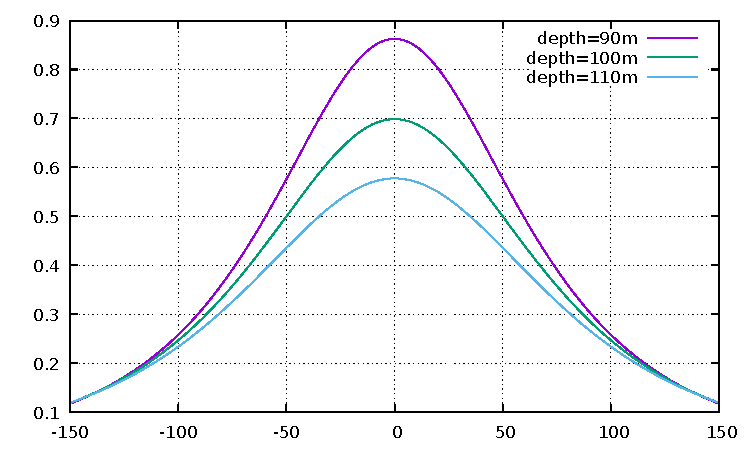
\includegraphics[width=6cm]{images/gravity/buriedsphere}
\end{center}

$g_z$ has its maximum value directly above the sphere at $x=0$m and is 
given by 
\[
g_{z}^{max}
= \frac{{\cal G} M_{sphere} d }{(d^2)^{3/2}}
= \frac{{\cal G} M_{sphere}  }{d^2}
\]
We can then find the half width of the curve by finding $x_{1/2}$ such that 
\[
\frac{{\cal G} M_{sphere} d }{(x_{1/2}^2 + d^2)^{3/2}} =
\frac{g_{z}^{max}}{2} = \frac{ {\cal G} M_{sphere} }{2 d^2}
\]
or, 
FINISH , derive $x_{1/2}$


%...............................................
\subsubsection{Buried horizontal cylinder (3D)} 

anticline can be approximated by a horizontal cylinder
\[
g_z=\frac{2 {\cal G} \pi a^2 d \Delta \rho}{x^2+d^2}
\]
the maximum value of g z is located directly above the axis of the cylinder

g zmax for a cylinder is larger than g zmax for a sphere of the same radius.

Cannot distinguish a buried sphere from a cylinder with just a single profile. Need to
collect gravity on a grid and make a map.

%............................
\subsubsection{Buried column (2D)}

\[
g_z=2 {\cal G} \Delta \rho b \ln \frac{r_2}{r_1}
\]

\begin{center}
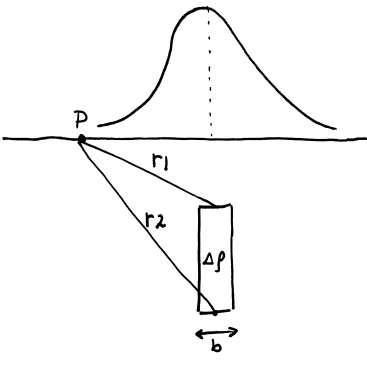
\includegraphics[width=3cm]{images/gravity/column}
\end{center}

%...................................
\subsubsection{Buried columns (2D)}

\[
g_z=2 {\cal G} \sum_i  \Delta \rho_i  b_i  \ln \frac{r_{2,i}}{r_{1,i}}
\]

\begin{center}
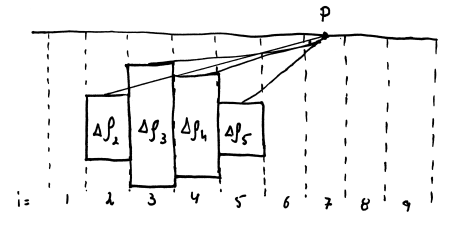
\includegraphics[width=3cm]{images/gravity/columns}
{\tiny {\color{gray} in ./images/gravity/columns/}}
\end{center}





%....................................
\subsubsection{Uniform layer of rock}

A layer of rock has an infinite extent, thickness $\Delta z$ 
and a density $\rho$. The gravitational
attraction of this slab at the point P at height $z$ obove the layer is 
\[
g_z=2 \pi {\cal G} \rho \Delta z
\]
Note that g z does not depend on the distance from the layer to the measurement point.



\newpage
%............................................................
\subsubsection{A constant density shell (Root \etal, 2021)}

Results \& raw data in {\tt ./images/benchmark\_gravity/bench1}

The shell is defined between $R_1$ and $R_2$. It contains a single material of 
density $3300\si{\kilogram\per\cubic\meter}$. The layer is centered around depth $100\si{\kilo\metre}$.
Gravity is measured $250\si{\kilo\metre}$ above the surface, i.e. $r=6621\si{\kilo\metre}$.
The thickness of the shell is 2, 5 or 10km.  

The analytical gravity vector norm is given by 
\[
g = \frac{4\pi}{3}\rho \frac{R_2^3-R_1^3}{r^2} {\cal G} 
\]
where we take ${\cal G}=6.67384\cdot10^{-11}$ (default in \aspect{}) or $\tilde{\cal G}=6.67428\cdot 10^{-11}$ sometimes.

\begin{center}
\begin{tabular}{lllll}
\hline
shell thickness      & volume                 & mass                & gravity using ${\cal G}$          & gravity using $\tilde{\cal G}$    \\
($\si{\kilo\metre}$) &  ($\si{\cubic\metre}$) & ($\si{\kilo\gram}$) & ($\si{\metre\per\square\second}$) & ($\si{\metre\per\square\second}$) \\
\hline\hline
2 & 9.8835614e17 & 3.2615753e21 & 496.542034795 &  496.574771345 \\
5 & 2.4708905e17 & 8.1539385e21 & 1241.35514223 & 1241.43698361 \\
10& 4.9417817e18 & 1.630788e22  & 2482.71067903 & 2482.87436182 \\
\hline
\end{tabular}
\end{center}    

In the \aspect{} input file there are three main parameters which may influence the results:
\begin{itemize}
\item the radial resolution, controlled in the input file by: {\tt set Number of slices = 1,2,3,4}
\item the tangential/lateral resolution, controlled by: {\tt set Initial lateral refinement  = 3,4,5,6}
\item the number of (additional) quadrature points, controlled by: {\tt set Quadrature degree increase =0,1,...6}
\end{itemize}
We set here the default values at 1, 6 and 3 respectively.

\begin{center}
\begin{tabular}{llllll}
\hline
         & lat. res. 3 & lat. res. 4 & lat. res. 5 & lat. res. 6 & lat. res. 7 \\ 
\hline
\hline
nslice=1 (1 cells radial) \# cells & 384   & 1,536 & 6,144  & 24,576 & 98,304  \\
           & $6\times64$  & $6\times256$ & $6\times1,024$ & $6\times4,096$ & $6\times16,384$ \\
           & $6\times8^2$  & $6\times16^2$ & $6\times32^2$ & $6\times64^2$ & $6\times128^2$ \\
nslice=2 (2 cells radial) \# cells & 768   & 3,072 & 12,288 & 49,152 & 196,608 \\
nslice=3 (3 cells radial) \# cells & 1,152 & 4,608 & 18,432 & 73,728 & 294,912 \\
nslice=4 (4 cells radial) \# cells & 1,536 & 6,144 & 24,576 & 98,304 & 393,216 \\
\hline
average area   (m2)   &  1.328292e+12 & 3.320732e11 & 8.30183e10 & 2.075457e10 & 5.188644e9 \\ 
approx size    (km)          &  1152km   & 576  & 288km & 144km  & 72km \\ 
approx size    (degree)      &  10.5 & 5.2 & 2.6 & 1.3 & 0.65 \\
\hline 
\end{tabular}
\end{center}

Earth has a surface of ${\cal S}=4\pi R^2\simeq 5.1006447\cdot 10^{14} \si{\square\meter}$. 
An average degree resolution means that this surface would be tesselated in blocks of 
approximately $2\pi R/ 360 \simeq 111\si{\kilo\metre}$ size. There would then be about 41,398 of such blocks. 
If a resolution of 2 degrees is required, then the blocks would be about 220km in size and 
there would be about 10,349 blocks. 

Results obtained with \aspect{} with $\tilde{G}$ are in the following table:

\noindent
\begin{tiny}
\begin{tabular}{|l|c|c|c|}
\hline
Thickness (km)  & 2   & 5  & 10 \\
Shell formula (mGal)  &  496.574771345 & 1241.43698361 & 2482.87436182 \\ 
\hline
$m=4$, $\sim{}5^\circ$   &  
496.554320/496.602897/496.574854 &
1241.385829/1241.507337/1241.437190 &
2482.771870/2483.015344/2482.874775 \\
$m=5$, $\sim{}2.6^\circ$ & 
496.574748/496.574819/496.574771 &
1241.436926/1241.437102/1241.436983 &
2482.874246/2482.874599/2482.874361 \\
$m=6$,$\sim{}1.3^\circ$  & 
496.574771/496.574771/496.574771 &
1241.436984/1241.436984/1241.436984 &
2482.874362/2482.874362/2482.874362 \\
\hline
\end{tabular}
\end{tiny}



%...................................................
\paragraph{Results for a 10km thick shell with \aspect{}}

\begin{center}
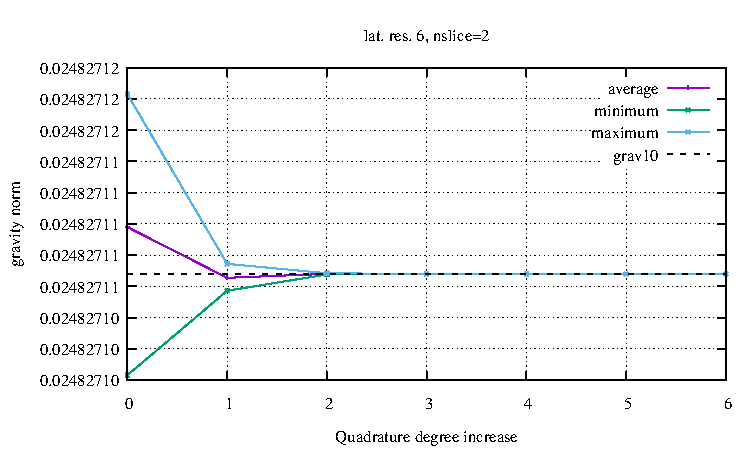
\includegraphics[width=5.7cm]{./images/benchmark_gravity/bench1/grav_nqplus}
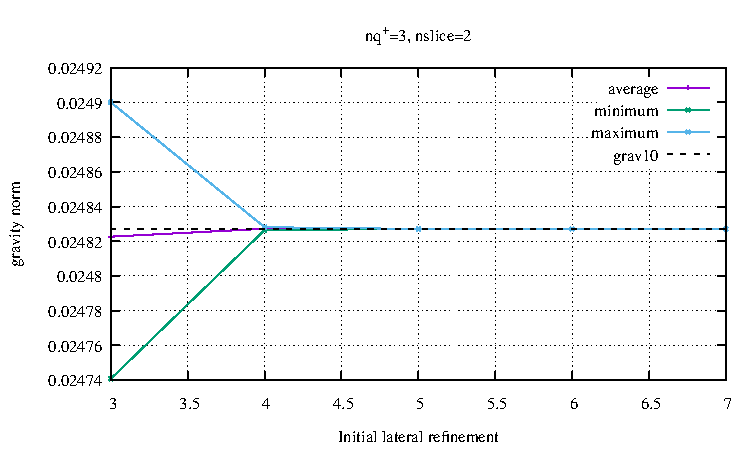
\includegraphics[width=5.7cm]{./images/benchmark_gravity/bench1/grav_latres}
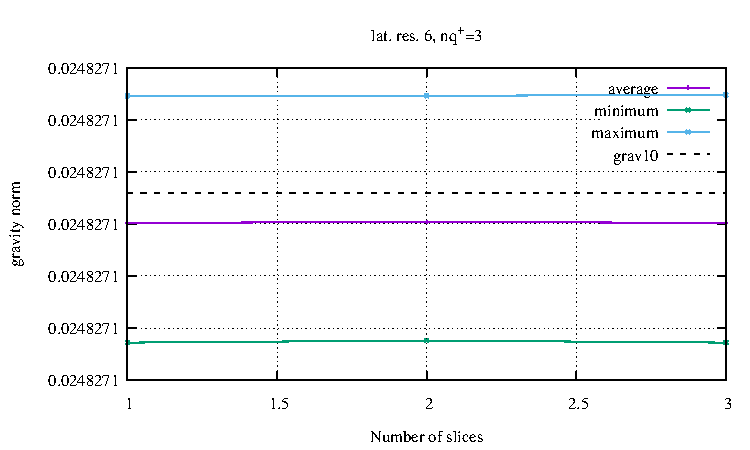
\includegraphics[width=5.7cm]{./images/benchmark_gravity/bench1/grav_nslice}\\
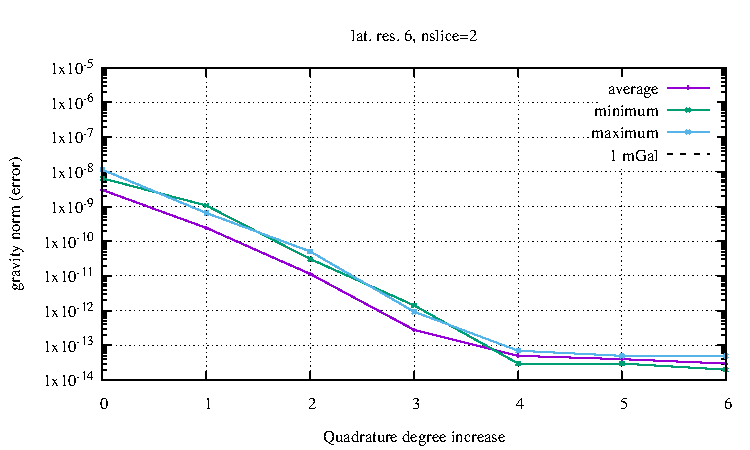
\includegraphics[width=5.7cm]{./images/benchmark_gravity/bench1/grav_nqplus_error}
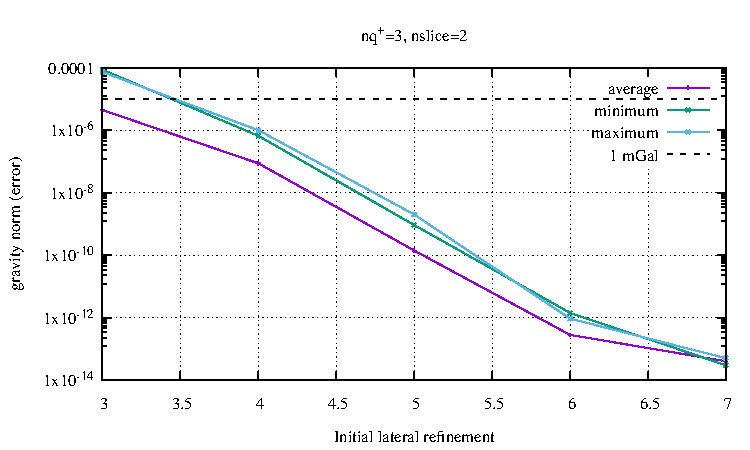
\includegraphics[width=5.7cm]{./images/benchmark_gravity/bench1/grav_latres_error}
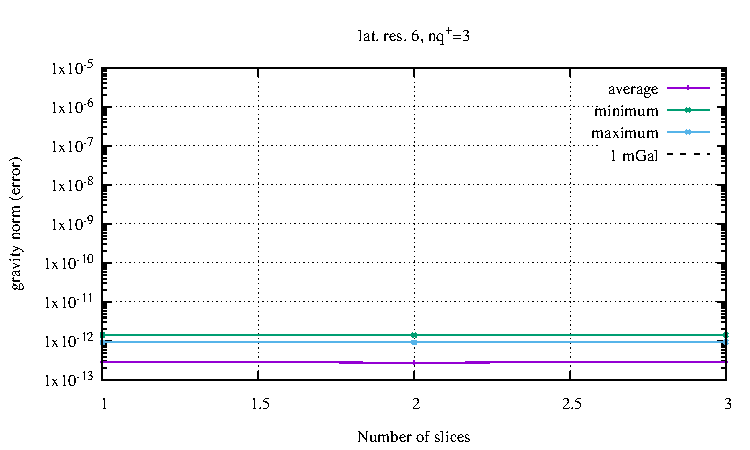
\includegraphics[width=5.7cm]{./images/benchmark_gravity/bench1/grav_nslice_error}\\
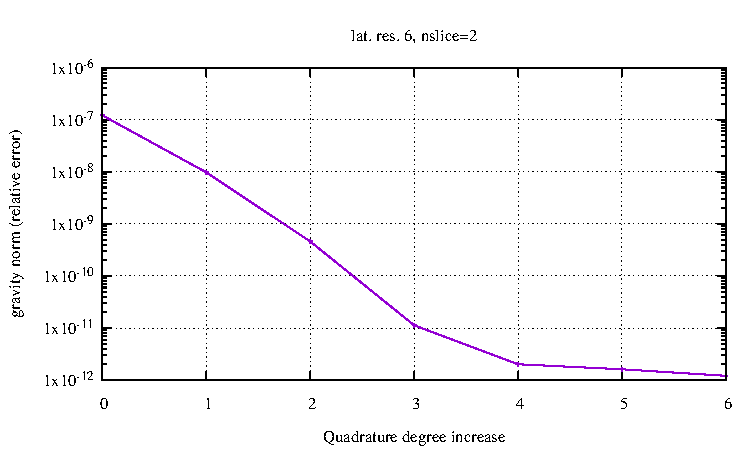
\includegraphics[width=5.7cm]{./images/benchmark_gravity/bench1/grav_nqplus_relerror}
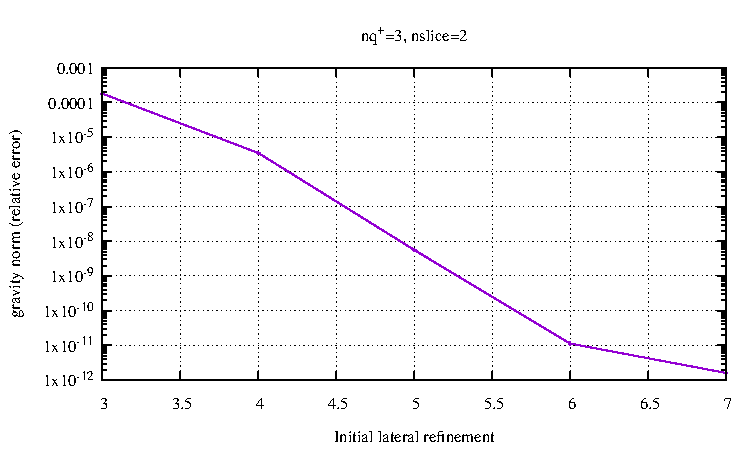
\includegraphics[width=5.7cm]{./images/benchmark_gravity/bench1/grav_latres_relerror}
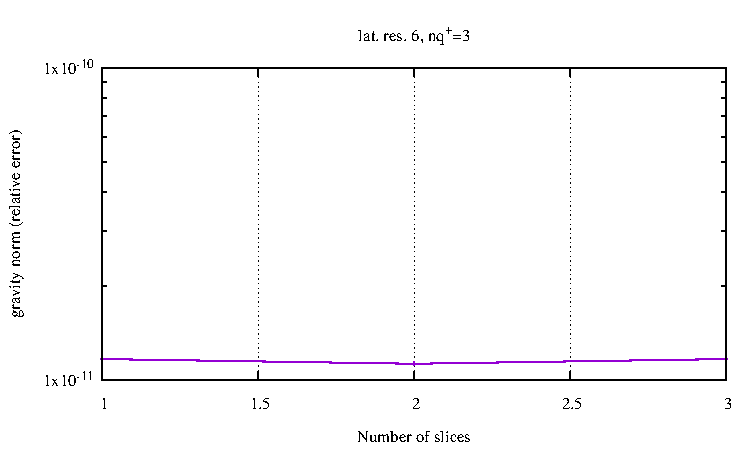
\includegraphics[width=5.7cm]{./images/benchmark_gravity/bench1/grav_nslice_relerror}\\
{\tiny {\color{gray} in ./images/benchmark\_gravity/bench1/}}
\end{center}

I then define the concept of 'cost'. In terms of computational cost, there is a tradeoff between resolution and 
number of quadrature points. The cost is then defined as 
\[
C = nel \times nq^3
\]
where $nel$ is the number of elements in the mesh and $nq$ is the number of quadrature points per element
and per dimension.


\begin{center}
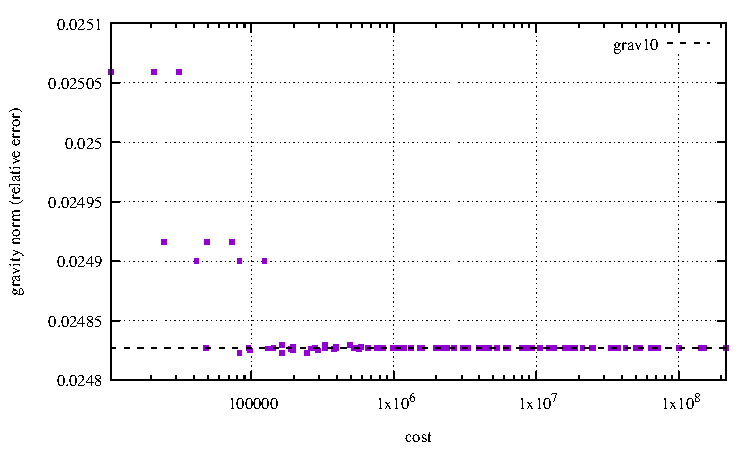
\includegraphics[width=5.7cm]{./images/benchmark_gravity/bench1/grav_cost}
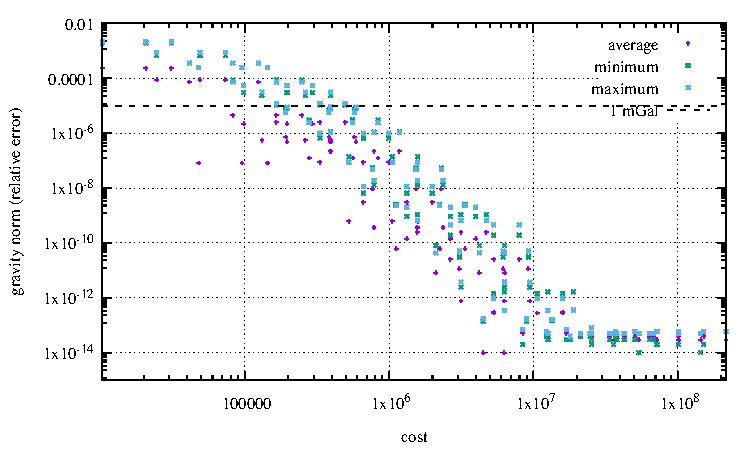
\includegraphics[width=5.7cm]{./images/benchmark_gravity/bench1/grav_cost_error}\\
{\tiny {\color{gray} in ./images/benchmark\_gravity/bench1/}}
\end{center}

Preliminary conclusion: nq+ at least 3, nslice not so important here, lat res at least 6


TODO RUN 2 and 5 km shells !


\newpage
%................................................
\subsubsection{The WINTERC mono-layer benchmark (Root \etal, 2021)}

A single data file is used,  {\tt rho\_56km\_SH\_W32.txt}, 
stored in {\tt images/benchmark\_gravity/bench2}. 
It contains density values for a single layer comprised between 56 and 80km depths, 
i.e. there is no radial variation of the density. 
Because of how \aspect{} works, the density values need to be transformed into 
initial temperatures. Using the simple material model we have
\[
\rho = \rho_0 (1-\alpha(T-T_0))
\]
so 
\[
T= \frac{1}{\alpha} \left(1 - \frac{\rho}{\rho_0} \right)
\]
and we here take $\alpha = 3\cdot 10^{-5}$, $T_0=0$ and $\rho_0=3300$, so that 
the temperatures range between -1198.9 and  141.5. These values make no sense, 
but all we want is that the densities $\rho(T)$ generated by the material model 
are those of the original dataset. 

Furthermore, the {\tt rho\_56km\_SH\_W32.txt} file contains 720x360 lines, i.e. 
the resolution is a half degree for longitude and latitude. These range from 0.25
to 359.75 and from -89.75 to 89.75 respectively. These must be transformed into 
spherical coordinates $\phi\in[0,2\pi]$ and $\theta \in[0,\pi]$.

Also the original data file contains longitude, latitude and density values for 
a thick layer. The ascii data file which \aspect can read requires radial values 
in increasing order as well, 
so for each combination $\phi-\theta$ I generate two values, one at 
radius 6371-81km and one at 6371-55km so that the depth layer 56-80km fits in it.
The data format of the ascii file is specified in 
{\tt data/initial-temperature/ascii-data/test/shell\_3d.txt} in \aspect{}.

Stone 98 reads in {\tt rho\_56km\_SH\_W32.txt} 
and generates the {\tt bench2.txt} file which is to be read by \aspect{}.
Note that the first line of this file is mandatory and reads: 
{\tt \# POINTS: 2 720 360}

\begin{center}
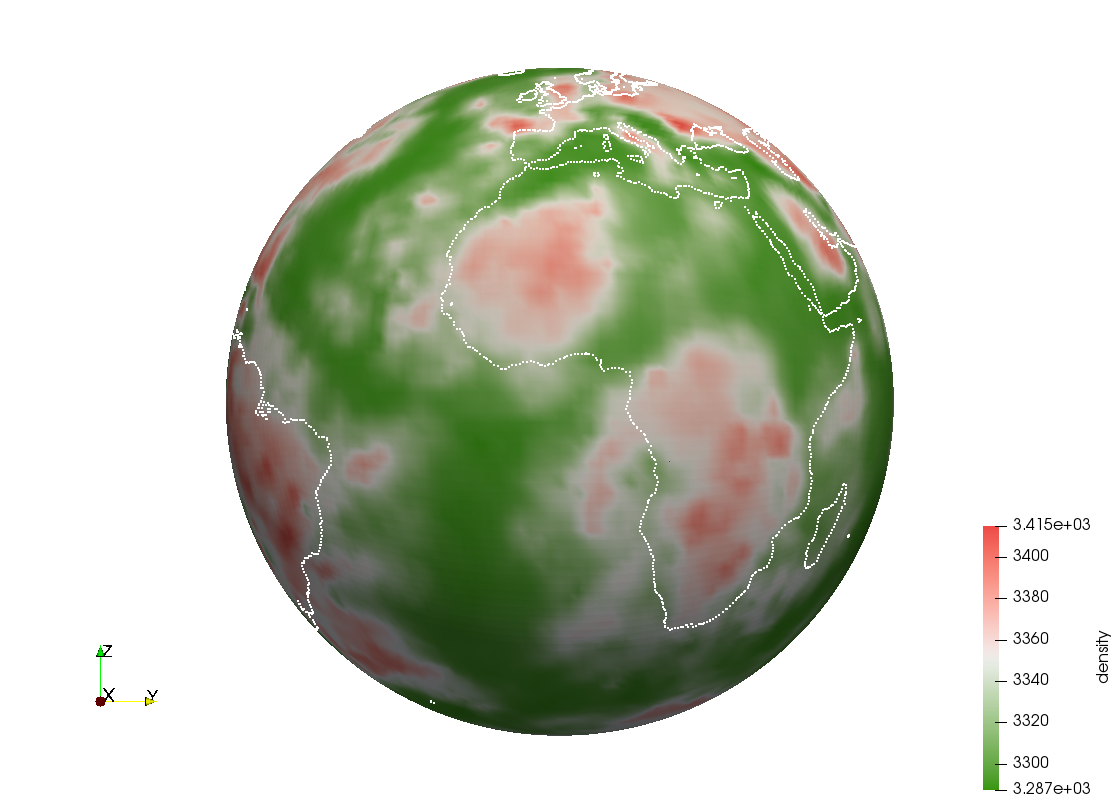
\includegraphics[width=5cm]{./images/benchmark_gravity/bench2/dens1}
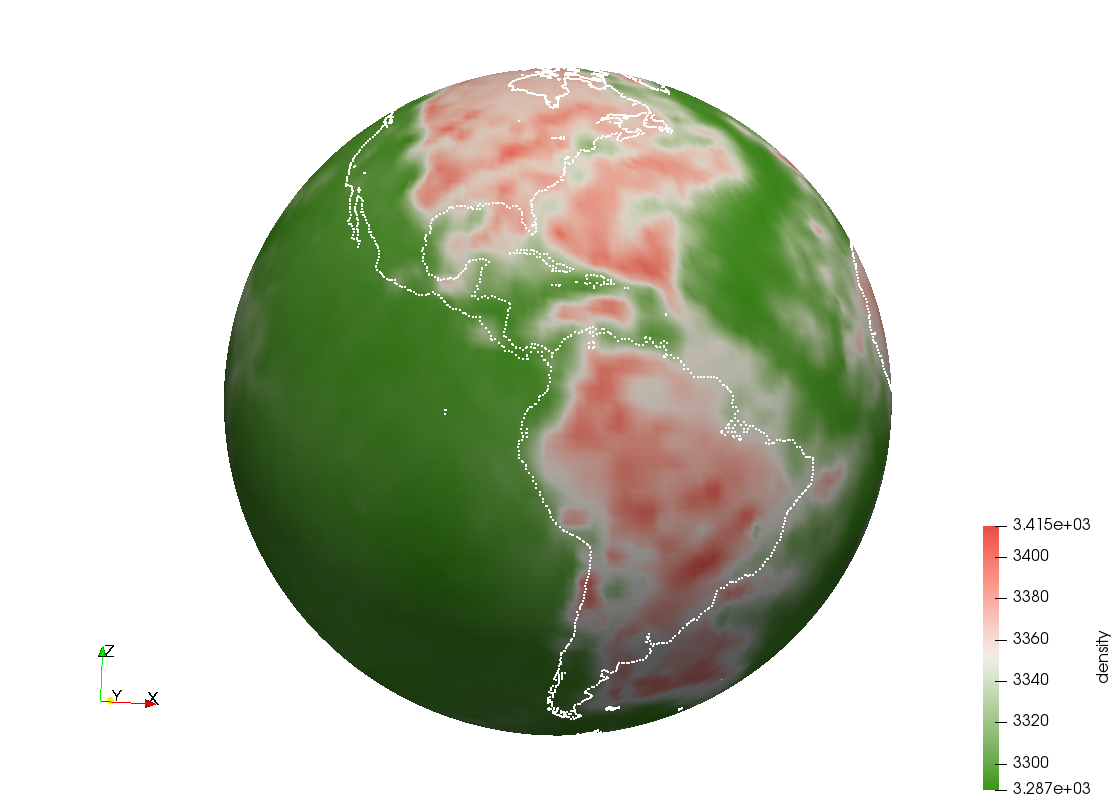
\includegraphics[width=5cm]{./images/benchmark_gravity/bench2/dens2}
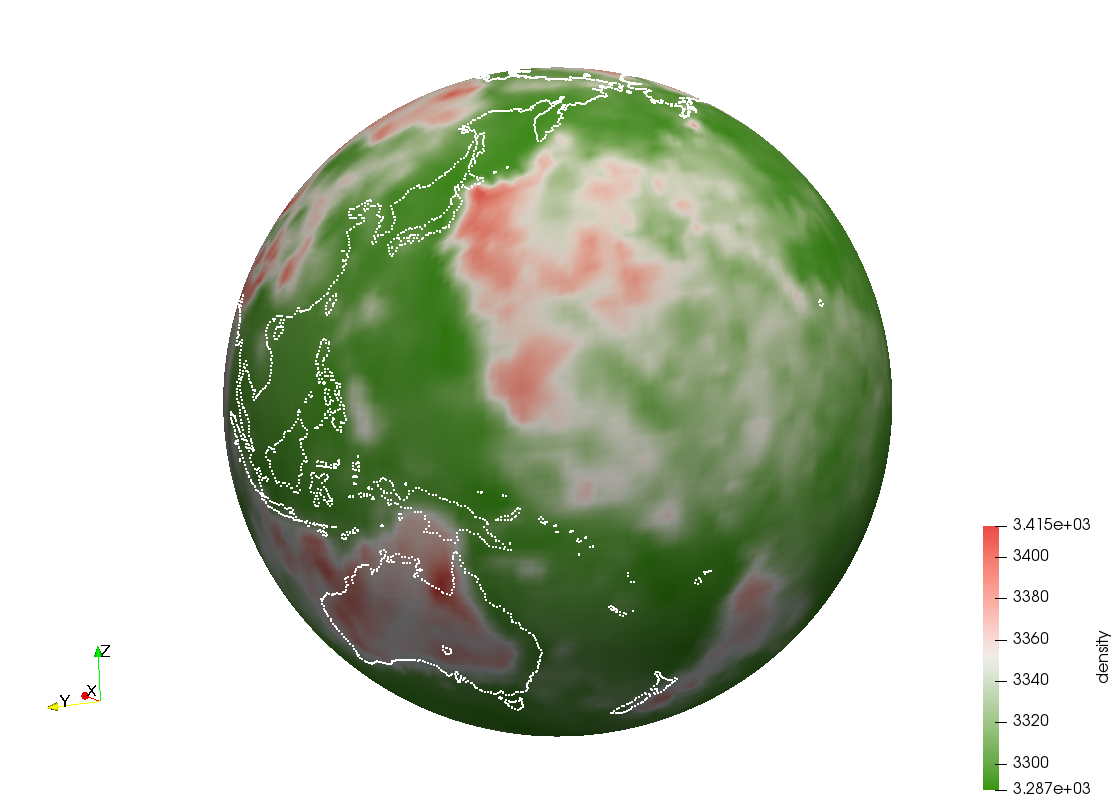
\includegraphics[width=5cm]{./images/benchmark_gravity/bench2/dens3}\\
{\tiny {\color{gray} in ./images/benchmark\_gravity/bench2/}}
\end{center}

\begin{center}
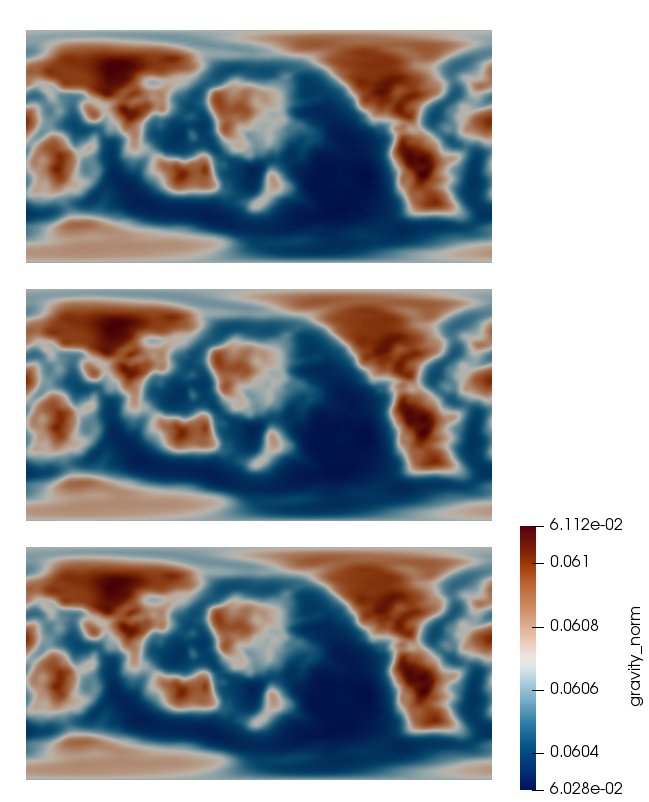
\includegraphics[width=7cm]{./images/benchmark_gravity/bench2/g}
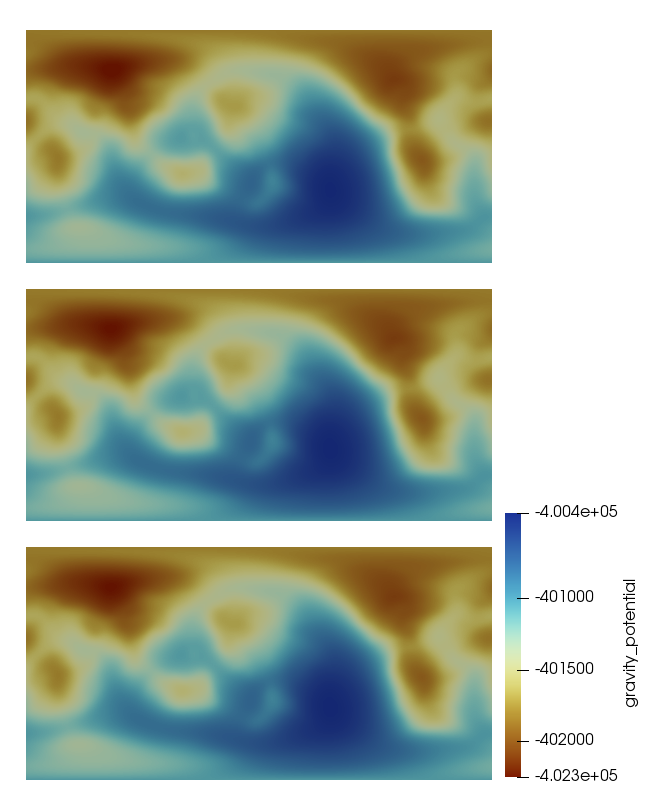
\includegraphics[width=7cm]{./images/benchmark_gravity/bench2/U}\\
{\captionfont Results obtained with \aspect{}. Top to bottom, level 4, 5, 6.
Measurements grid is 181x91 points.\\
{\tiny {\color{gray} in ./images/benchmark\_gravity/bench2/}}
}
\end{center}

\begin{center}
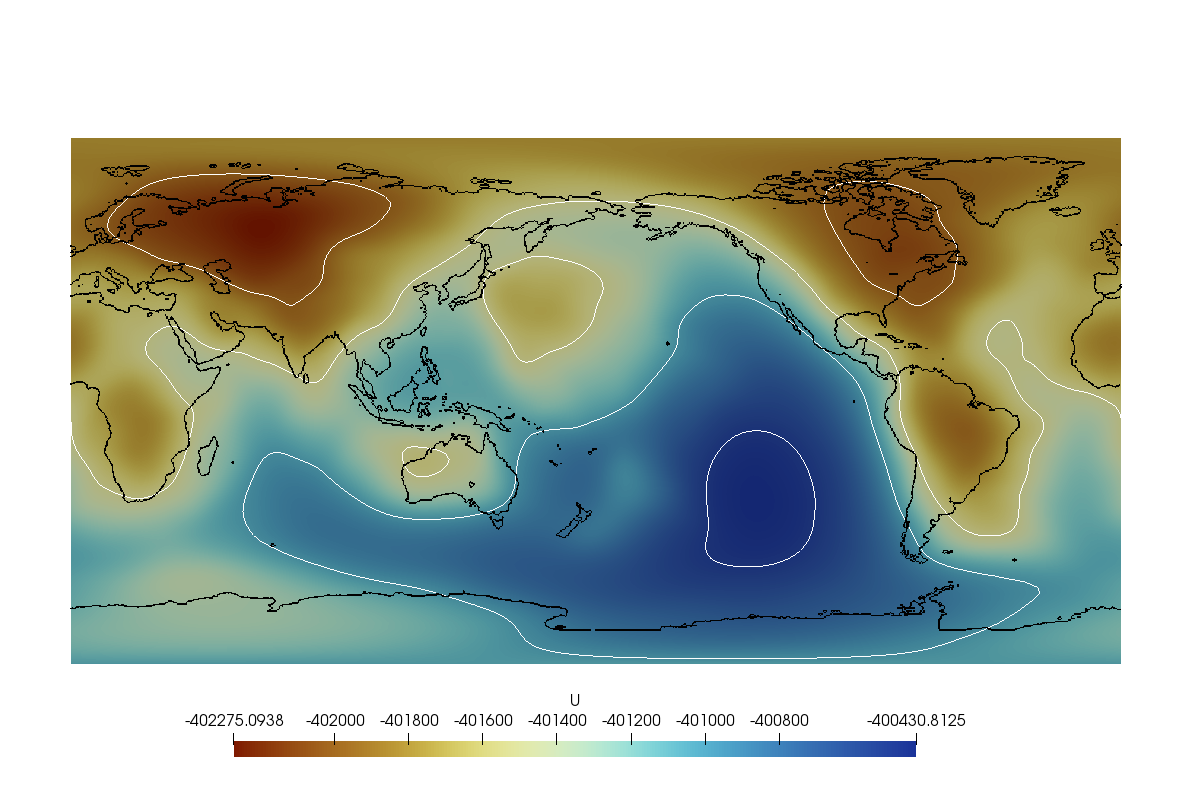
\includegraphics[width=8.5cm]{python_codes/fieldstone_98/images/U}
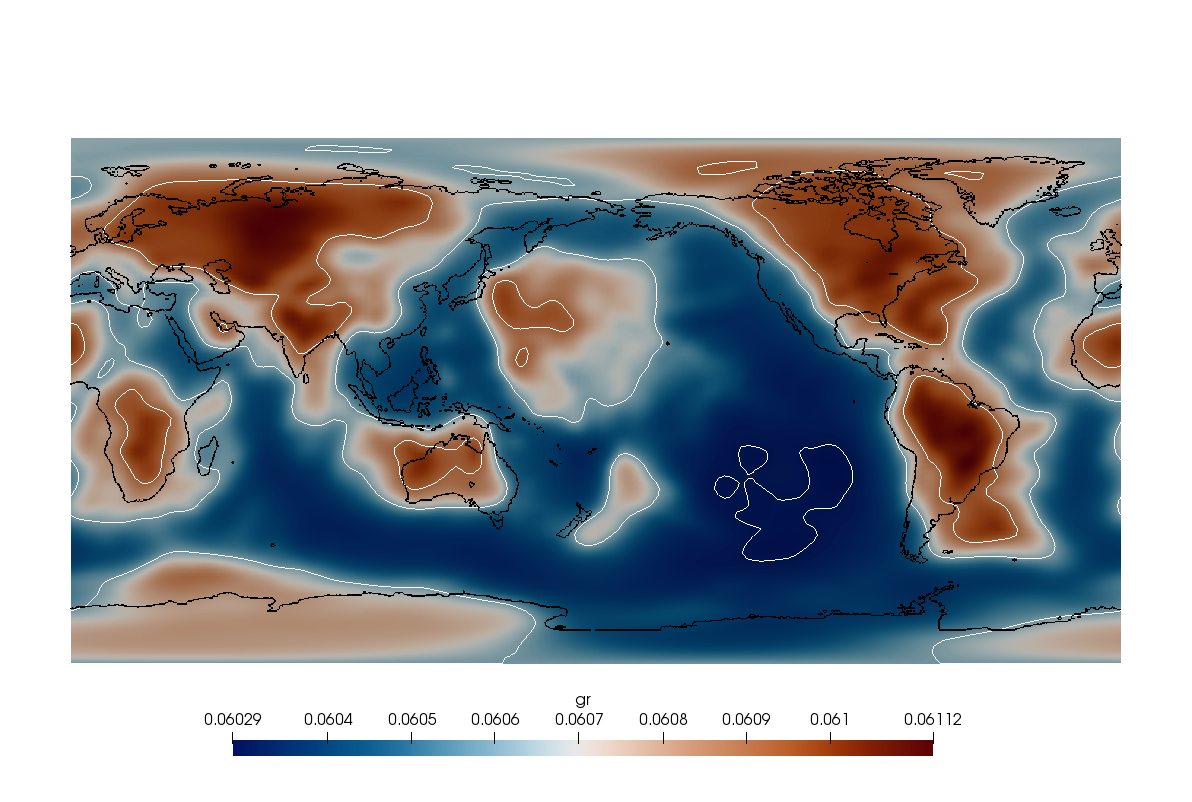
\includegraphics[width=8.5cm]{python_codes/fieldstone_98/images/gr}\\
{\captionfont From Stone 98. Resolution of measurement grid is 181x91. It took 
about 19,100 seconds to run, averaging 1.16s per measurement point.  
Potential isocontours at -400.5e3, -401e3, -401.5e3, -402e3. 
Radial acceleration contours at 0.0603, 0.0606 and 0.0609.\\
{\tiny {\color{gray} in ./python\_codes/images/}}
}
\end{center}

\begin{tabular}{lcccc}
\hline
level & avrg density & total mass & number of cells & time \\
\hline
\hline
4     & 3323  & 3.981e+22 & 1,536  & 503s  \\
5     & 3323  & 3.981e+22 & 6,144  & 2030s \\
6     & 3323  & 3.981e+22 & 24.576 & 8190s \\
\hline
\end{tabular}

\newpage
%....................................
\subsubsection{Moho benchmark (Root \etal, 2021)}

We consider an 80km thick shell with a density interface inside, using CRUST1.0 Moho 
for the boundary (upper dens = 2900kg/m3, lower dens = 3300 kg/m3).
Stone 97 reads the CRUST1.0 file and transforms it into {\tt bench3.ascii} in the 
right ASPECT format.  


\begin{center}
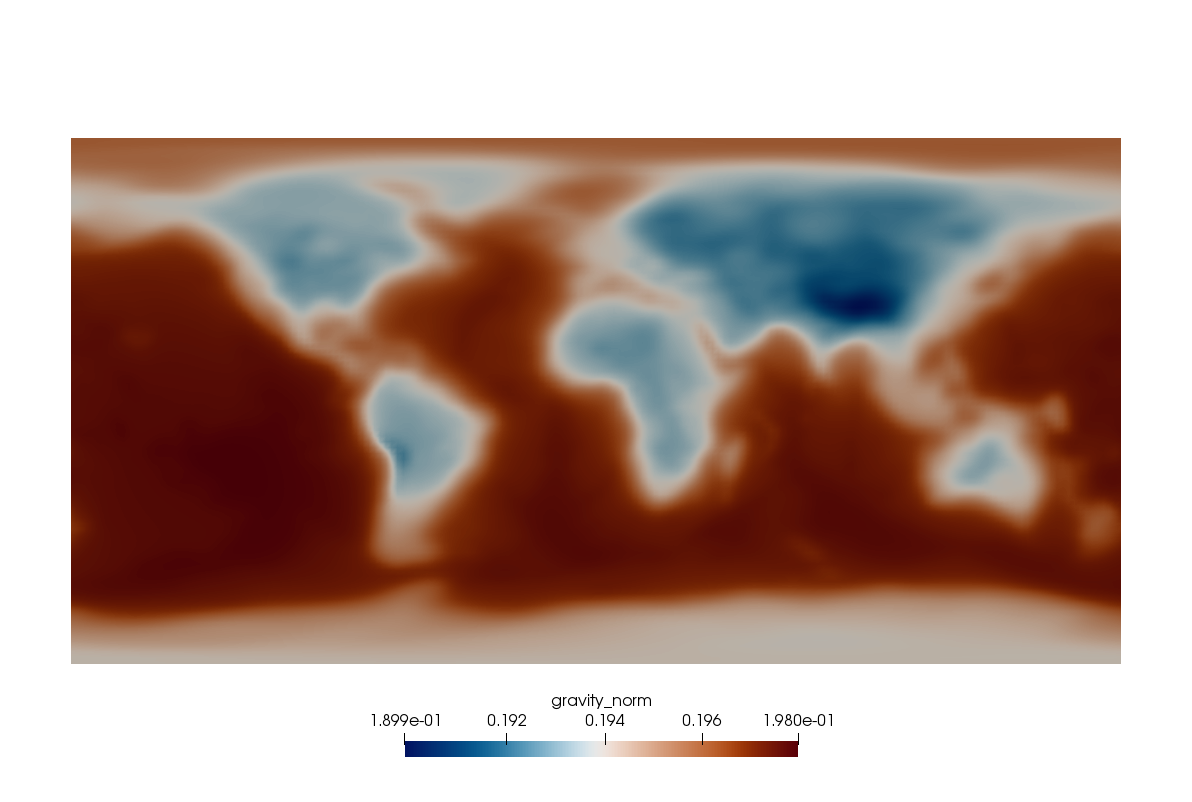
\includegraphics[width=7.5cm]{./images/benchmark_gravity/bench3/g}
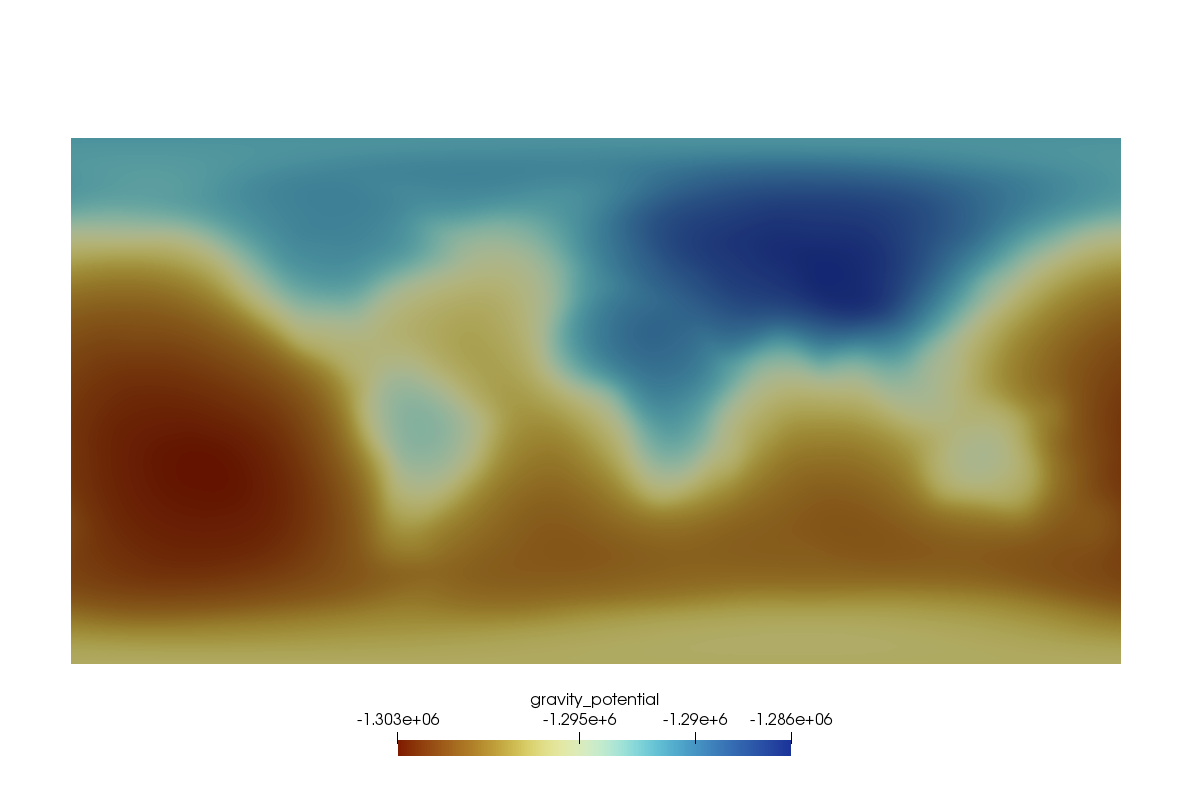
\includegraphics[width=7.5cm]{./images/benchmark_gravity/bench3/U}\\
{\captionfont bench3.ascii file has 301 points in the radial direction, i.e. a 
300m resolution. 181x91 gravity measurement points. Lateral refinement level is 6, 25 slices.\\
{\tiny {\color{gray} in ./images/benchmark\_gravity/bench3/}}
}
\end{center}




